\documentclass[11pt]{article}
\usepackage[textwidth=18.0cm, textheight=23.0cm, top=2.0cm]{geometry}
\usepackage{pst-all}
\usepackage{amssymb}
\usepackage{tikz}
\usepackage{underscore}\begin{document}
\pagestyle{empty}


ClassName: \underline{\textbf{Class_07.2bp-15}}
\par
BinSize: \underline{\textbf{100 × 100}}
\par
ReduceSize: \underline{\textbf{100 × 100}}
\par
TypeNum: \underline{\textbf{40}}
\par
Num: \underline{\textbf{40}}
\par
OutS: \underline{\textbf{110000}}
\par
InS: \underline{\textbf{95584}}
\par
Rate: \underline{\textbf{0.869}}
\par
UB: \underline{\textbf{11}}
\par
LB0: \underline{\textbf{11}}
\par
LB: \underline{\textbf{11}}
\par
LBWithCut: \underline{\textbf{11}}
\par
NodeCut: \underline{\textbf{0}}
\par
ExtendedNodeCnt: \underline{\textbf{1}}
\par
GenNodeCnt: \underline{\textbf{1}}
\par
PrimalNode: \underline{\textbf{0}}
\par
ColumnCount: \underline{\textbf{11}}
\par
TotalCutCount: \underline{\textbf{0}}
\par
RootCutCount: \underline{\textbf{0}}
\par
LPSolverCnt: \underline{\textbf{1}}
\par
PricingSolverCnt: \underline{\textbf{0}}
\par
BranchAndBoundNum: \underline{\textbf{1}}
\par
isOpt: \underline{\textbf{true}}
\par
TimeOnInitSolution: \underline{\textbf{600.000 s}}
\par
TimeOnPrimal: \underline{\textbf{0.000 s}}
\par
TimeOnPricing: \underline{\textbf{0.000 s}}
\par
TimeOnRmp: \underline{\textbf{0.125 s}}
\par
TotalTime: \underline{\textbf{600.422 s}}
\par
\newpage


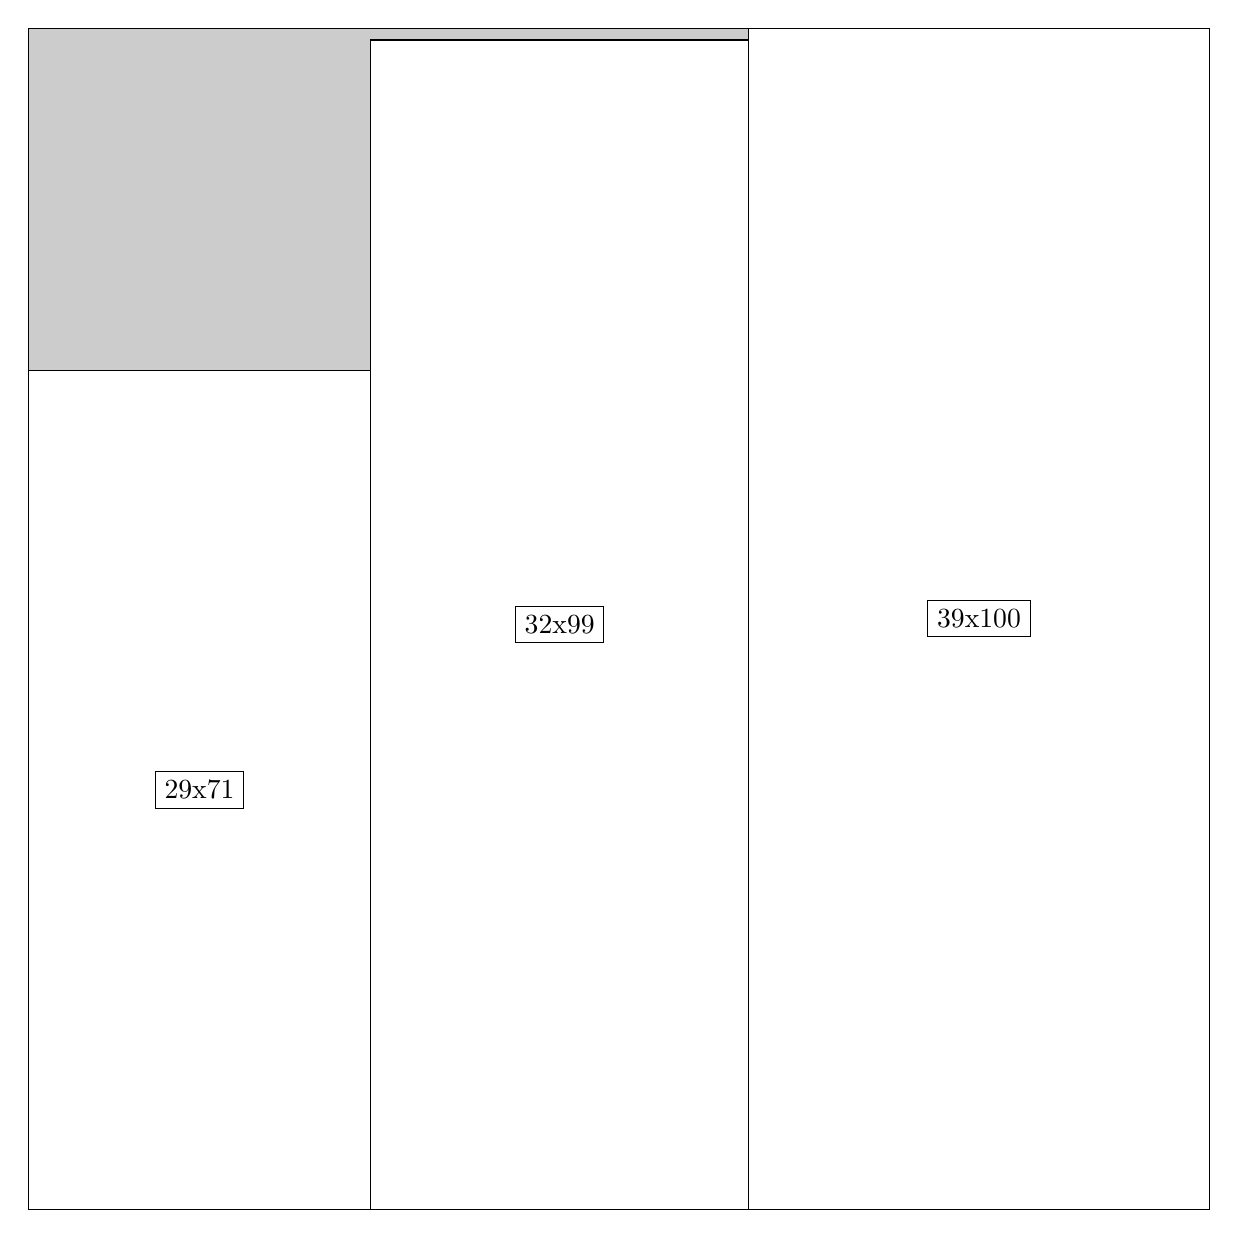
\begin{tikzpicture}[shorten >=1pt,scale=1.0,every node/.style={scale=1.0},->]
\tikzstyle{vertex}=[circle,fill=black!25,minimum size=14pt,inner sep=0pt]
\filldraw[fill=gray!40!white, draw=black] (0,0) rectangle (15.0,15.0);
\foreach \name/\x/\y/\w/\h in {39x100/9.15/0.0/5.85/15.0,32x99/4.35/0.0/4.8/14.85,29x71/0.0/0.0/4.35/10.65}
\filldraw[fill=white!40!white, draw=black] (\x,\y) rectangle node[draw] (\name) {\name} ++(\w,\h);
\end{tikzpicture}


w =39 , h =100 , x =61 , y =0 , v =3900
\par
w =32 , h =99 , x =29 , y =0 , v =3168
\par
w =29 , h =71 , x =0 , y =0 , v =2059
\par
\newpage


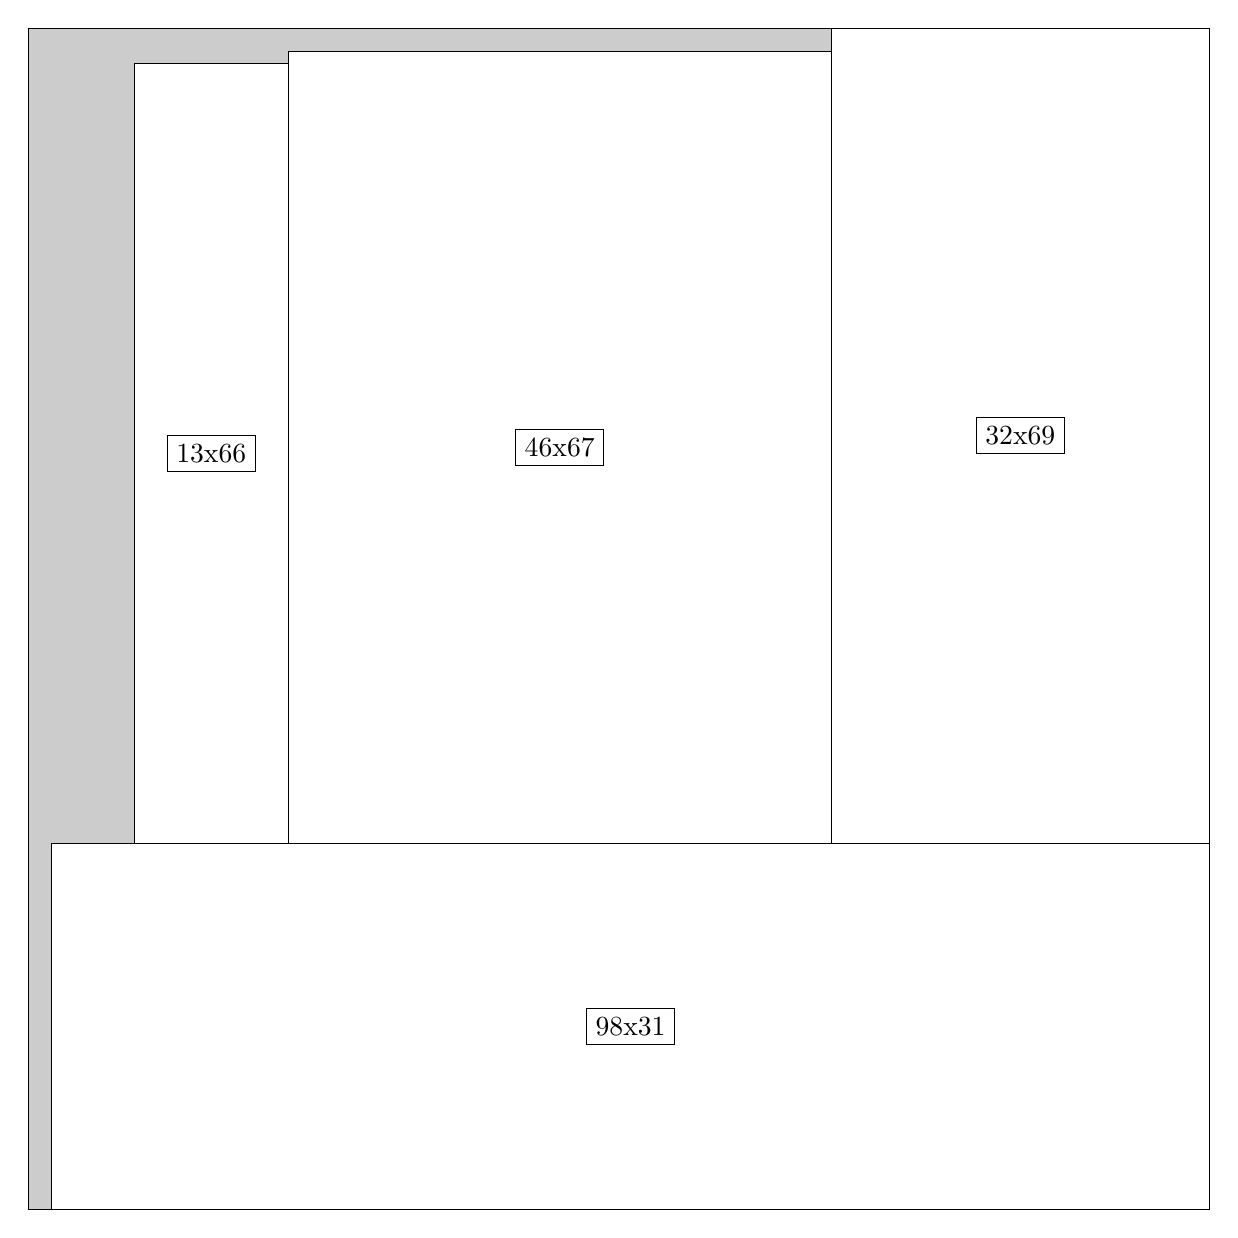
\begin{tikzpicture}[shorten >=1pt,scale=1.0,every node/.style={scale=1.0},->]
\tikzstyle{vertex}=[circle,fill=black!25,minimum size=14pt,inner sep=0pt]
\filldraw[fill=gray!40!white, draw=black] (0,0) rectangle (15.0,15.0);
\foreach \name/\x/\y/\w/\h in {98x31/0.3/0.0/14.7/4.6499999999999995,32x69/10.2/4.6499999999999995/4.8/10.35,46x67/3.3/4.6499999999999995/6.8999999999999995/10.049999999999999,13x66/1.3499999999999999/4.6499999999999995/1.95/9.9}
\filldraw[fill=white!40!white, draw=black] (\x,\y) rectangle node[draw] (\name) {\name} ++(\w,\h);
\end{tikzpicture}


w =98 , h =31 , x =2 , y =0 , v =3038
\par
w =32 , h =69 , x =68 , y =31 , v =2208
\par
w =46 , h =67 , x =22 , y =31 , v =3082
\par
w =13 , h =66 , x =9 , y =31 , v =858
\par
\newpage


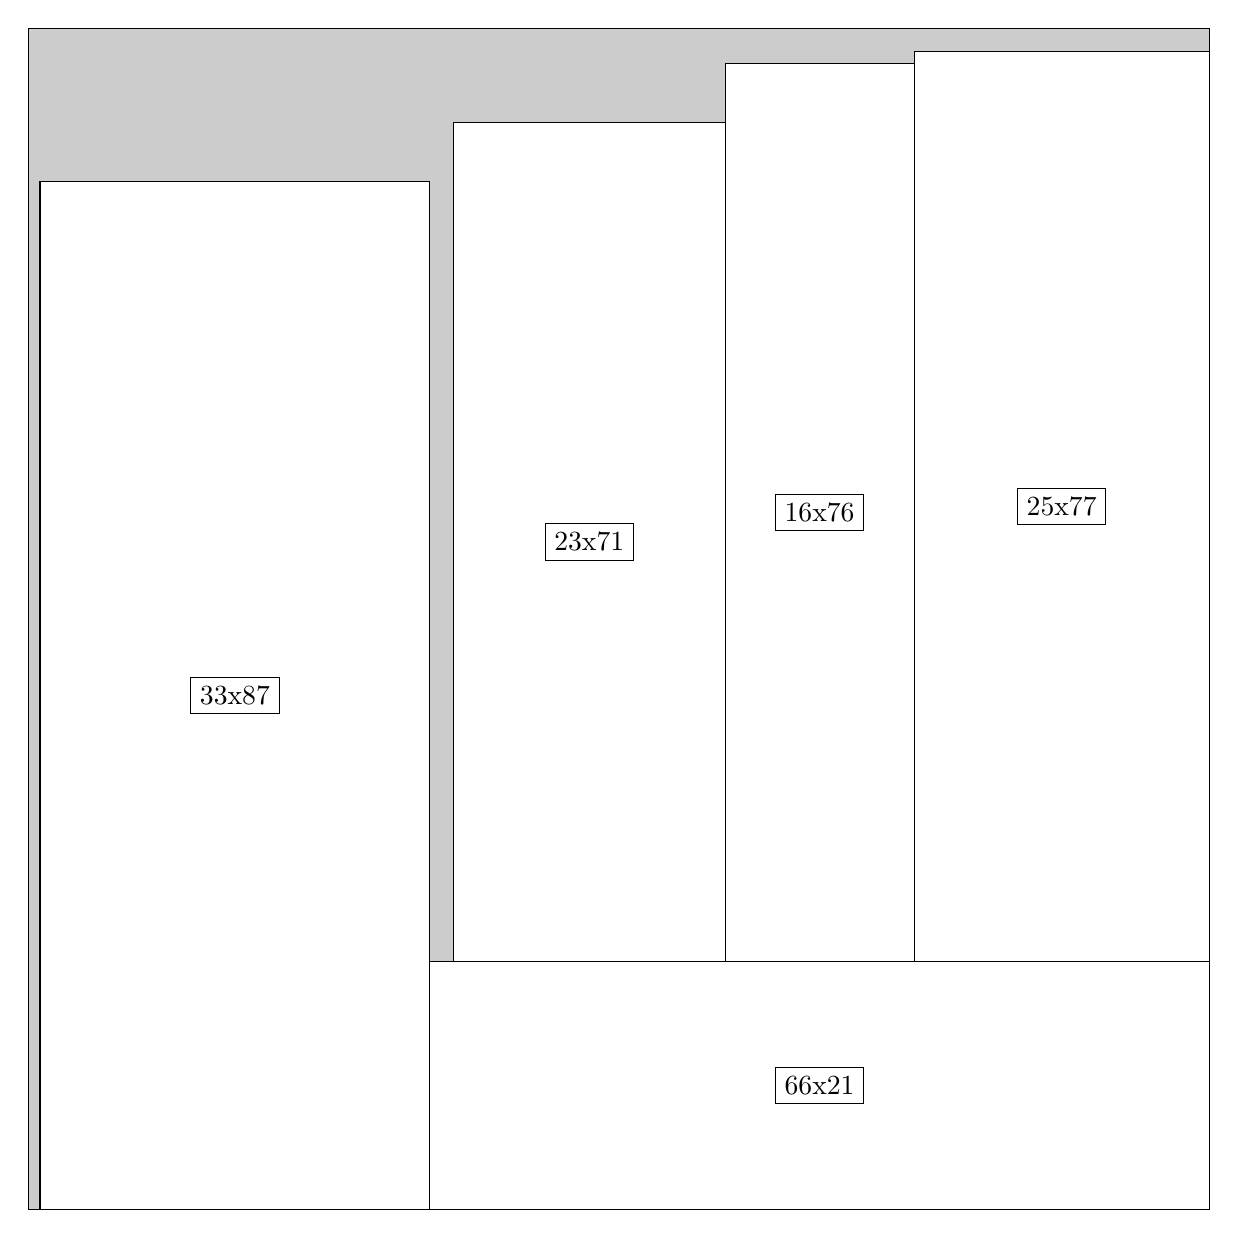
\begin{tikzpicture}[shorten >=1pt,scale=1.0,every node/.style={scale=1.0},->]
\tikzstyle{vertex}=[circle,fill=black!25,minimum size=14pt,inner sep=0pt]
\filldraw[fill=gray!40!white, draw=black] (0,0) rectangle (15.0,15.0);
\foreach \name/\x/\y/\w/\h in {66x21/5.1/0.0/9.9/3.15,25x77/11.25/3.15/3.75/11.549999999999999,16x76/8.85/3.15/2.4/11.4,23x71/5.3999999999999995/3.15/3.4499999999999997/10.65,33x87/0.15/0.0/4.95/13.049999999999999}
\filldraw[fill=white!40!white, draw=black] (\x,\y) rectangle node[draw] (\name) {\name} ++(\w,\h);
\end{tikzpicture}


w =66 , h =21 , x =34 , y =0 , v =1386
\par
w =25 , h =77 , x =75 , y =21 , v =1925
\par
w =16 , h =76 , x =59 , y =21 , v =1216
\par
w =23 , h =71 , x =36 , y =21 , v =1633
\par
w =33 , h =87 , x =1 , y =0 , v =2871
\par
\newpage


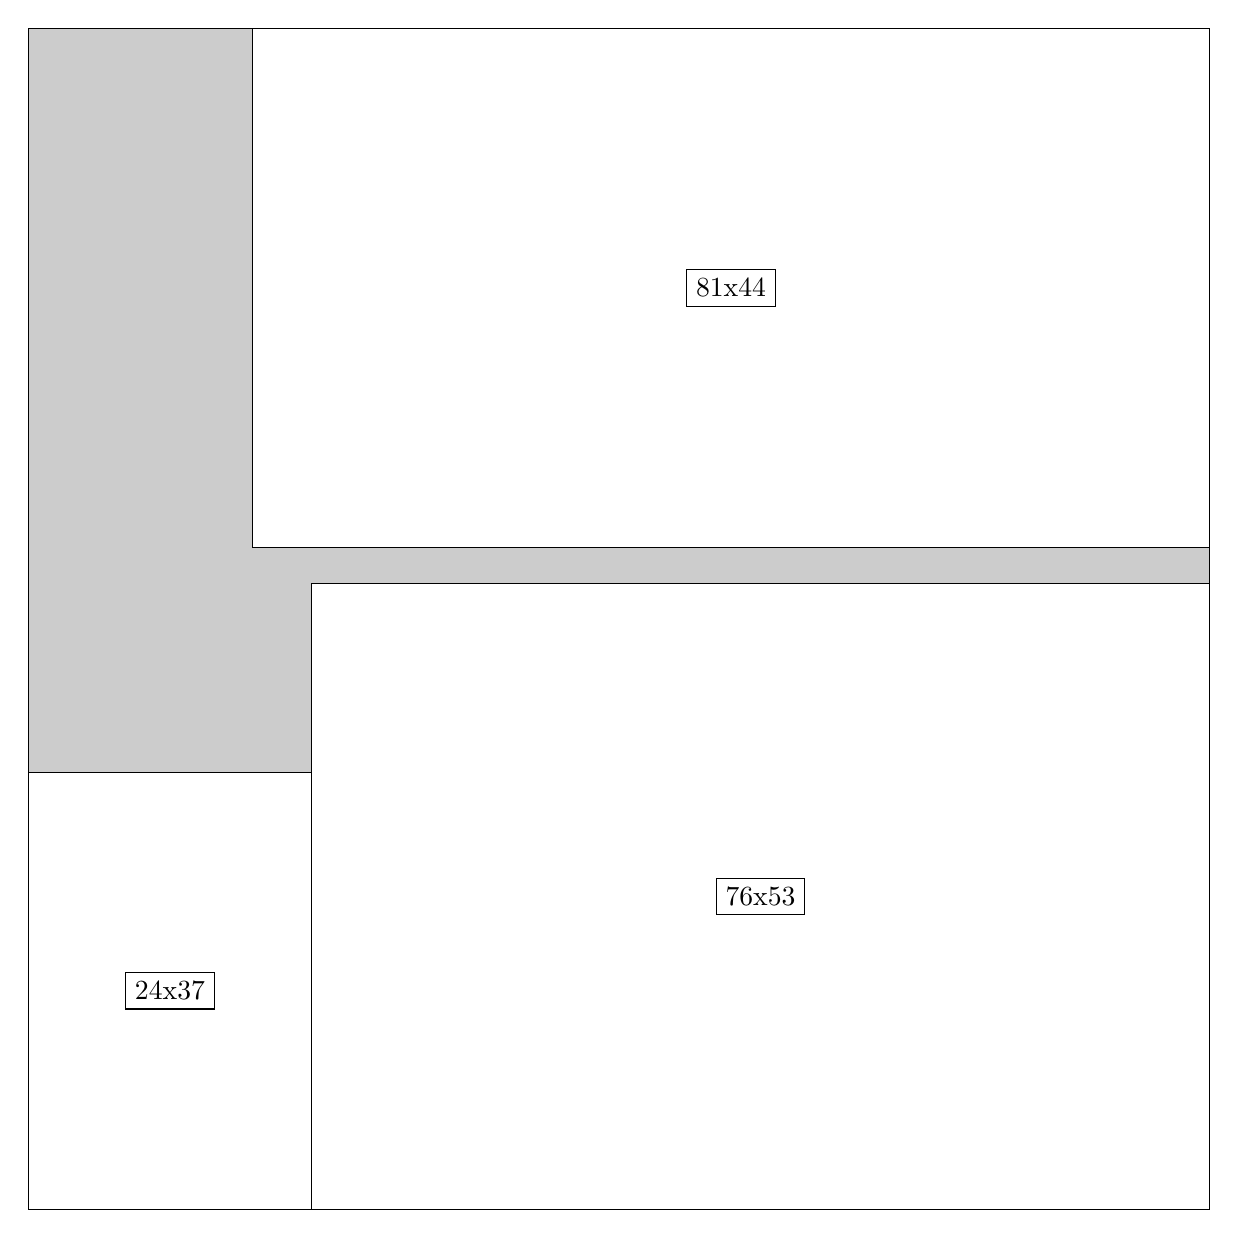
\begin{tikzpicture}[shorten >=1pt,scale=1.0,every node/.style={scale=1.0},->]
\tikzstyle{vertex}=[circle,fill=black!25,minimum size=14pt,inner sep=0pt]
\filldraw[fill=gray!40!white, draw=black] (0,0) rectangle (15.0,15.0);
\foreach \name/\x/\y/\w/\h in {76x53/3.5999999999999996/0.0/11.4/7.949999999999999,24x37/0.0/0.0/3.5999999999999996/5.55,81x44/2.85/8.4/12.15/6.6}
\filldraw[fill=white!40!white, draw=black] (\x,\y) rectangle node[draw] (\name) {\name} ++(\w,\h);
\end{tikzpicture}


w =76 , h =53 , x =24 , y =0 , v =4028
\par
w =24 , h =37 , x =0 , y =0 , v =888
\par
w =81 , h =44 , x =19 , y =56 , v =3564
\par
\newpage


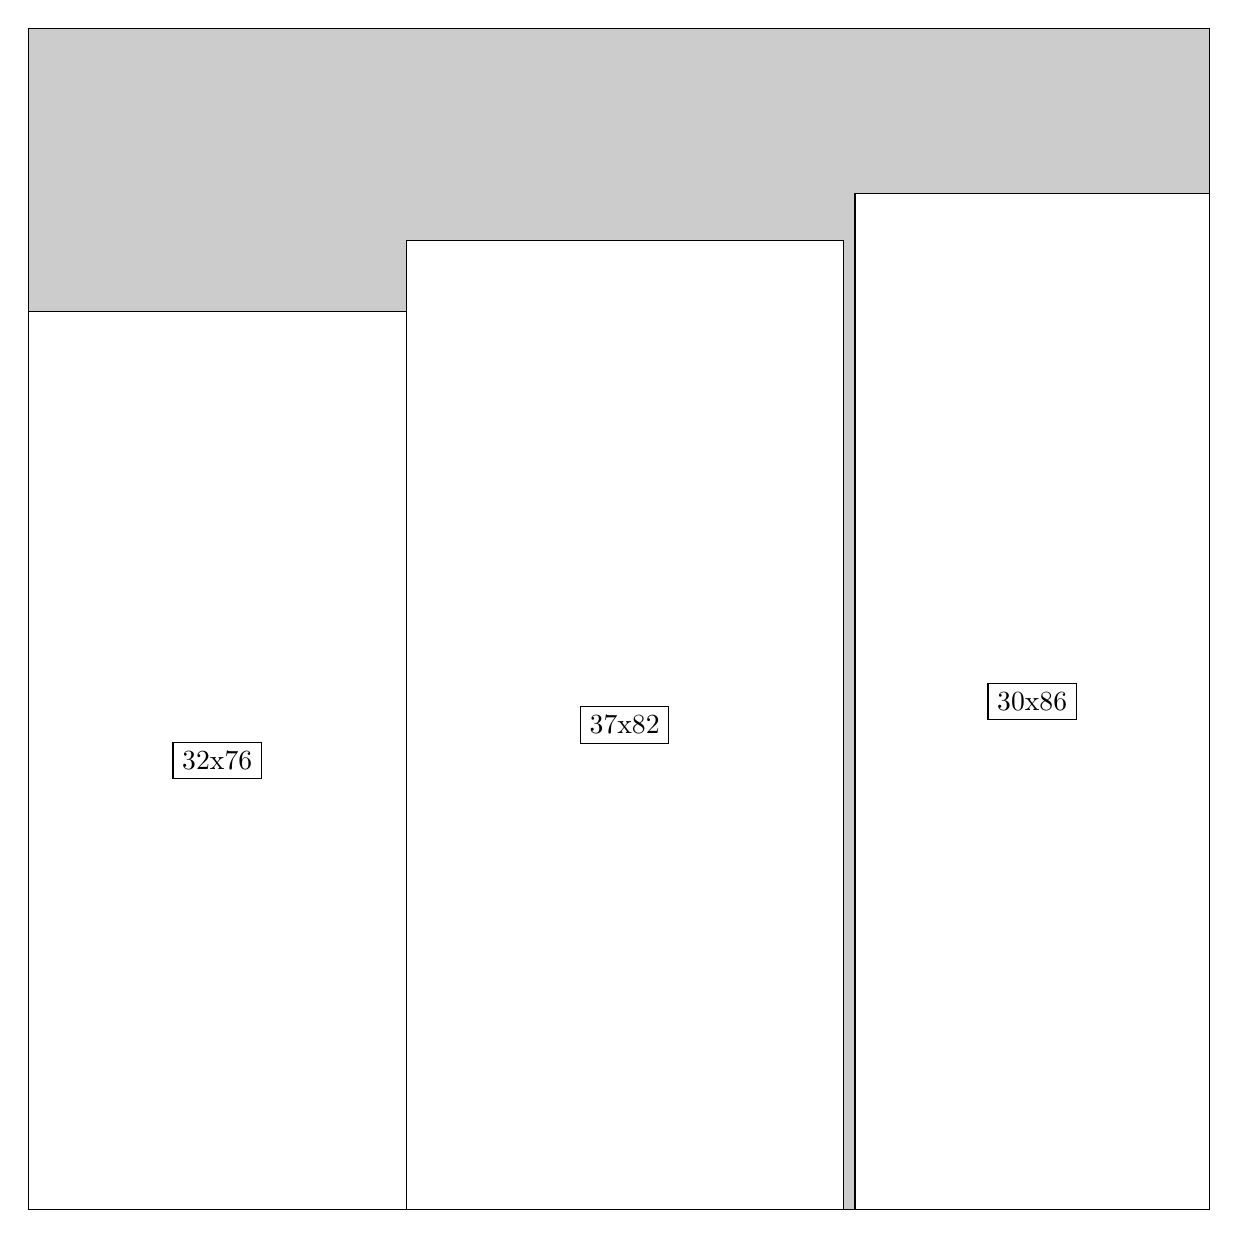
\begin{tikzpicture}[shorten >=1pt,scale=1.0,every node/.style={scale=1.0},->]
\tikzstyle{vertex}=[circle,fill=black!25,minimum size=14pt,inner sep=0pt]
\filldraw[fill=gray!40!white, draw=black] (0,0) rectangle (15.0,15.0);
\foreach \name/\x/\y/\w/\h in {30x86/10.5/0.0/4.5/12.9,37x82/4.8/0.0/5.55/12.299999999999999,32x76/0.0/0.0/4.8/11.4}
\filldraw[fill=white!40!white, draw=black] (\x,\y) rectangle node[draw] (\name) {\name} ++(\w,\h);
\end{tikzpicture}


w =30 , h =86 , x =70 , y =0 , v =2580
\par
w =37 , h =82 , x =32 , y =0 , v =3034
\par
w =32 , h =76 , x =0 , y =0 , v =2432
\par
\newpage


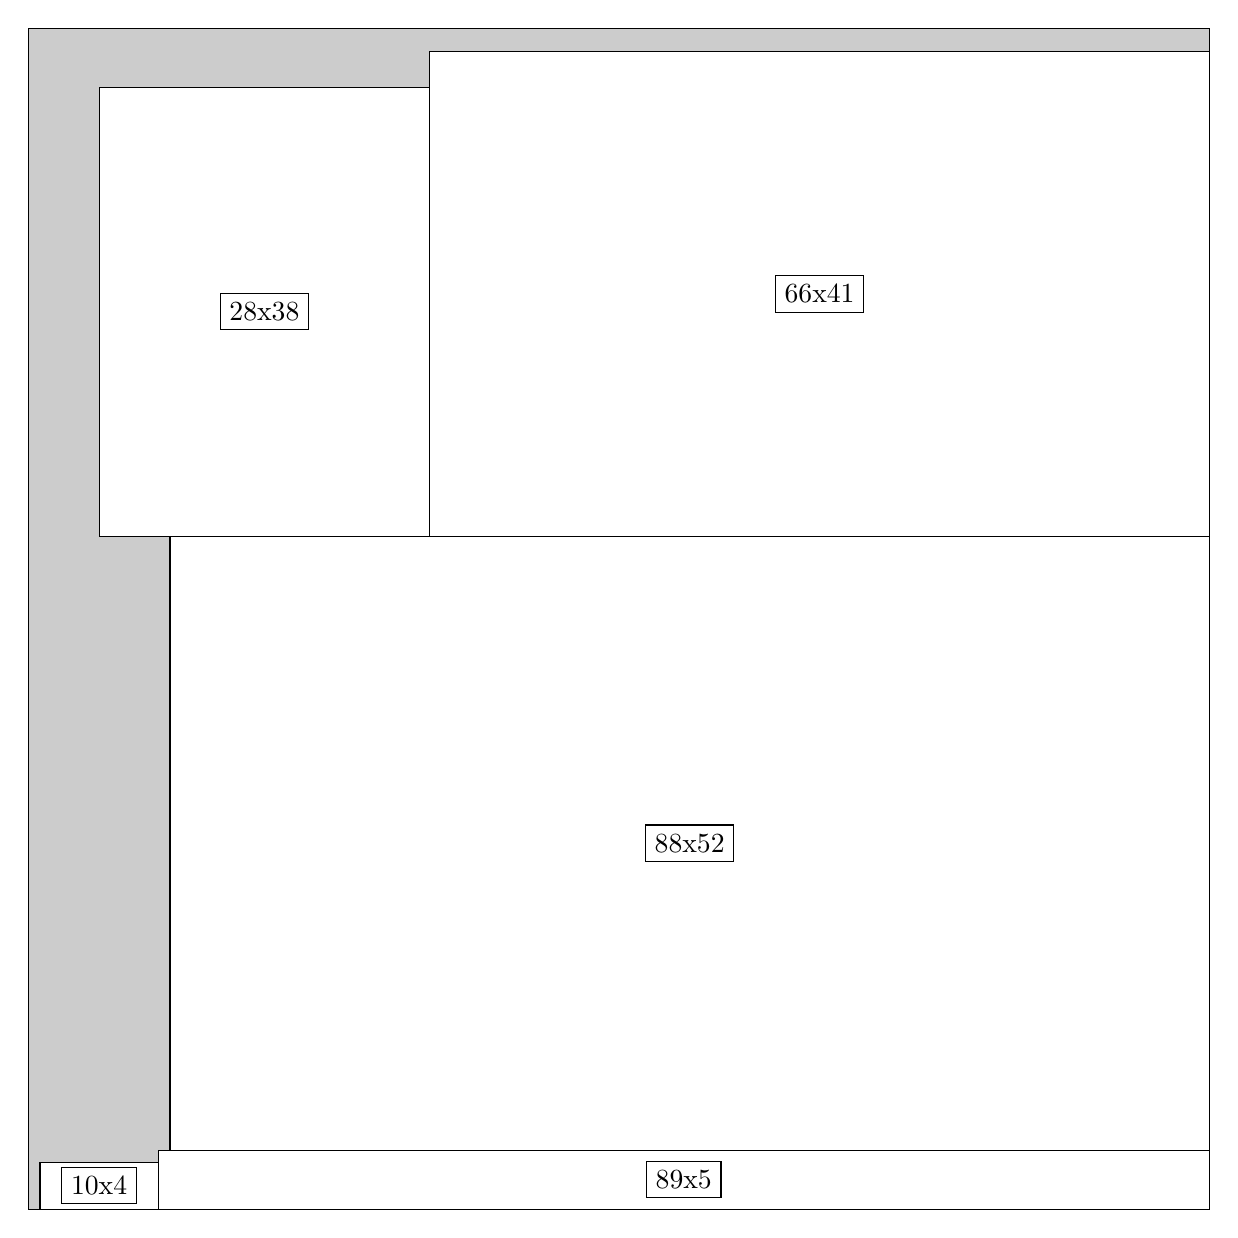
\begin{tikzpicture}[shorten >=1pt,scale=1.0,every node/.style={scale=1.0},->]
\tikzstyle{vertex}=[circle,fill=black!25,minimum size=14pt,inner sep=0pt]
\filldraw[fill=gray!40!white, draw=black] (0,0) rectangle (15.0,15.0);
\foreach \name/\x/\y/\w/\h in {89x5/1.65/0.0/13.35/0.75,10x4/0.15/0.0/1.5/0.6,88x52/1.7999999999999998/0.75/13.2/7.8,66x41/5.1/8.549999999999999/9.9/6.1499999999999995,28x38/0.8999999999999999/8.549999999999999/4.2/5.7}
\filldraw[fill=white!40!white, draw=black] (\x,\y) rectangle node[draw] (\name) {\name} ++(\w,\h);
\end{tikzpicture}


w =89 , h =5 , x =11 , y =0 , v =445
\par
w =10 , h =4 , x =1 , y =0 , v =40
\par
w =88 , h =52 , x =12 , y =5 , v =4576
\par
w =66 , h =41 , x =34 , y =57 , v =2706
\par
w =28 , h =38 , x =6 , y =57 , v =1064
\par
\newpage


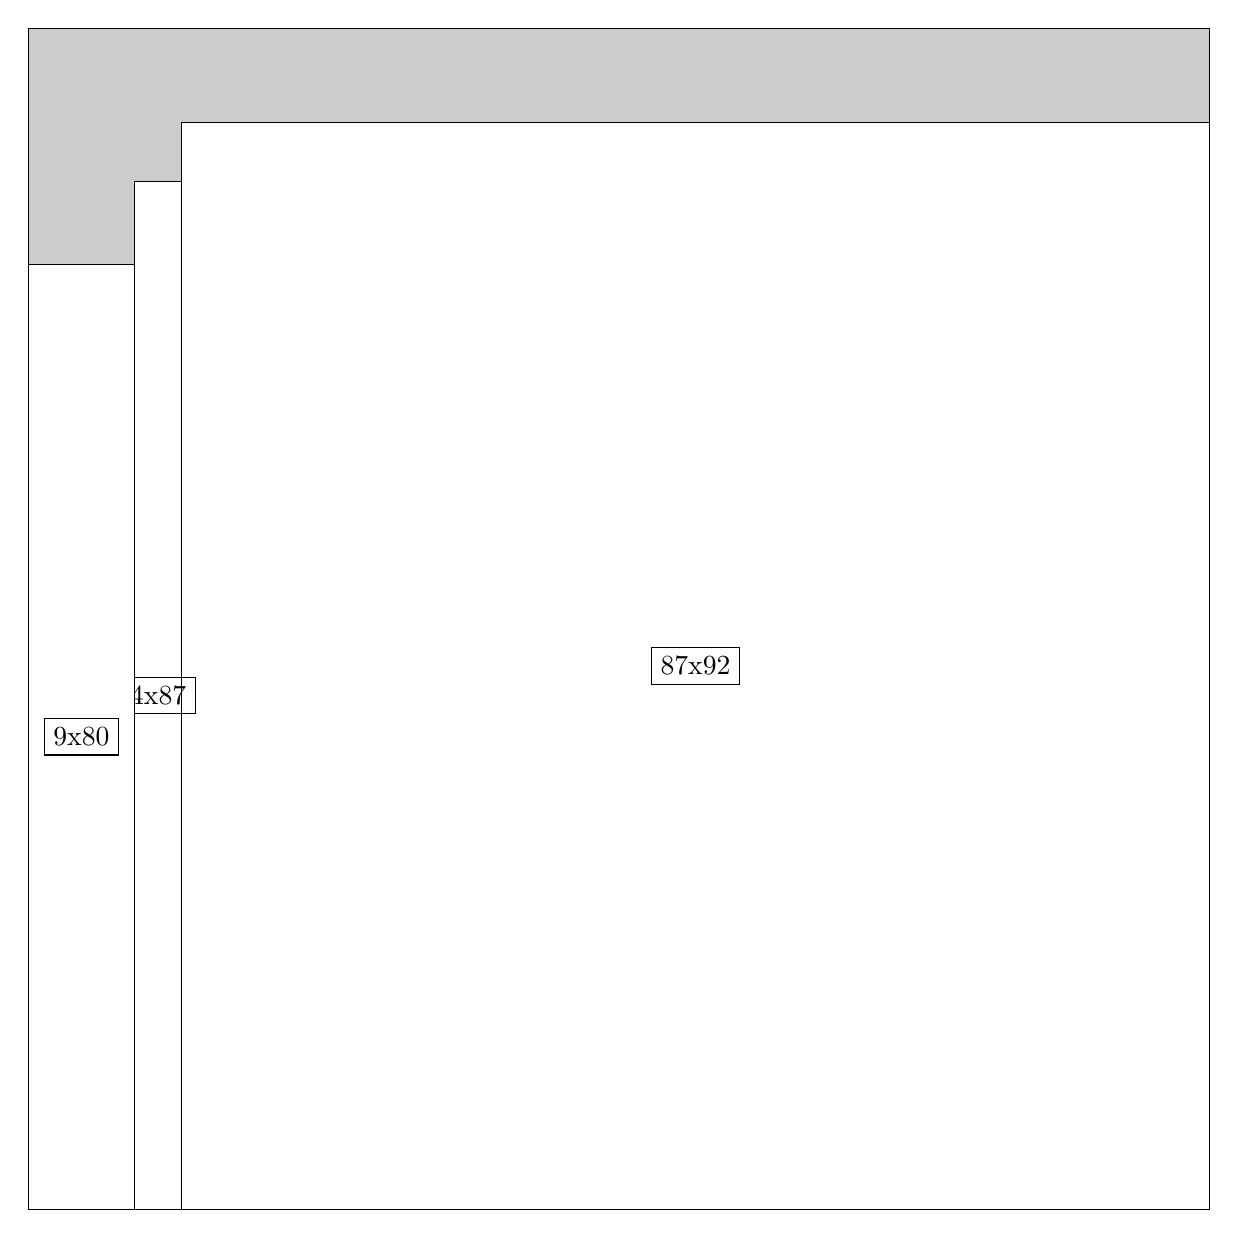
\begin{tikzpicture}[shorten >=1pt,scale=1.0,every node/.style={scale=1.0},->]
\tikzstyle{vertex}=[circle,fill=black!25,minimum size=14pt,inner sep=0pt]
\filldraw[fill=gray!40!white, draw=black] (0,0) rectangle (15.0,15.0);
\foreach \name/\x/\y/\w/\h in {87x92/1.95/0.0/13.049999999999999/13.799999999999999,4x87/1.3499999999999999/0.0/0.6/13.049999999999999,9x80/0.0/0.0/1.3499999999999999/12.0}
\filldraw[fill=white!40!white, draw=black] (\x,\y) rectangle node[draw] (\name) {\name} ++(\w,\h);
\end{tikzpicture}


w =87 , h =92 , x =13 , y =0 , v =8004
\par
w =4 , h =87 , x =9 , y =0 , v =348
\par
w =9 , h =80 , x =0 , y =0 , v =720
\par
\newpage


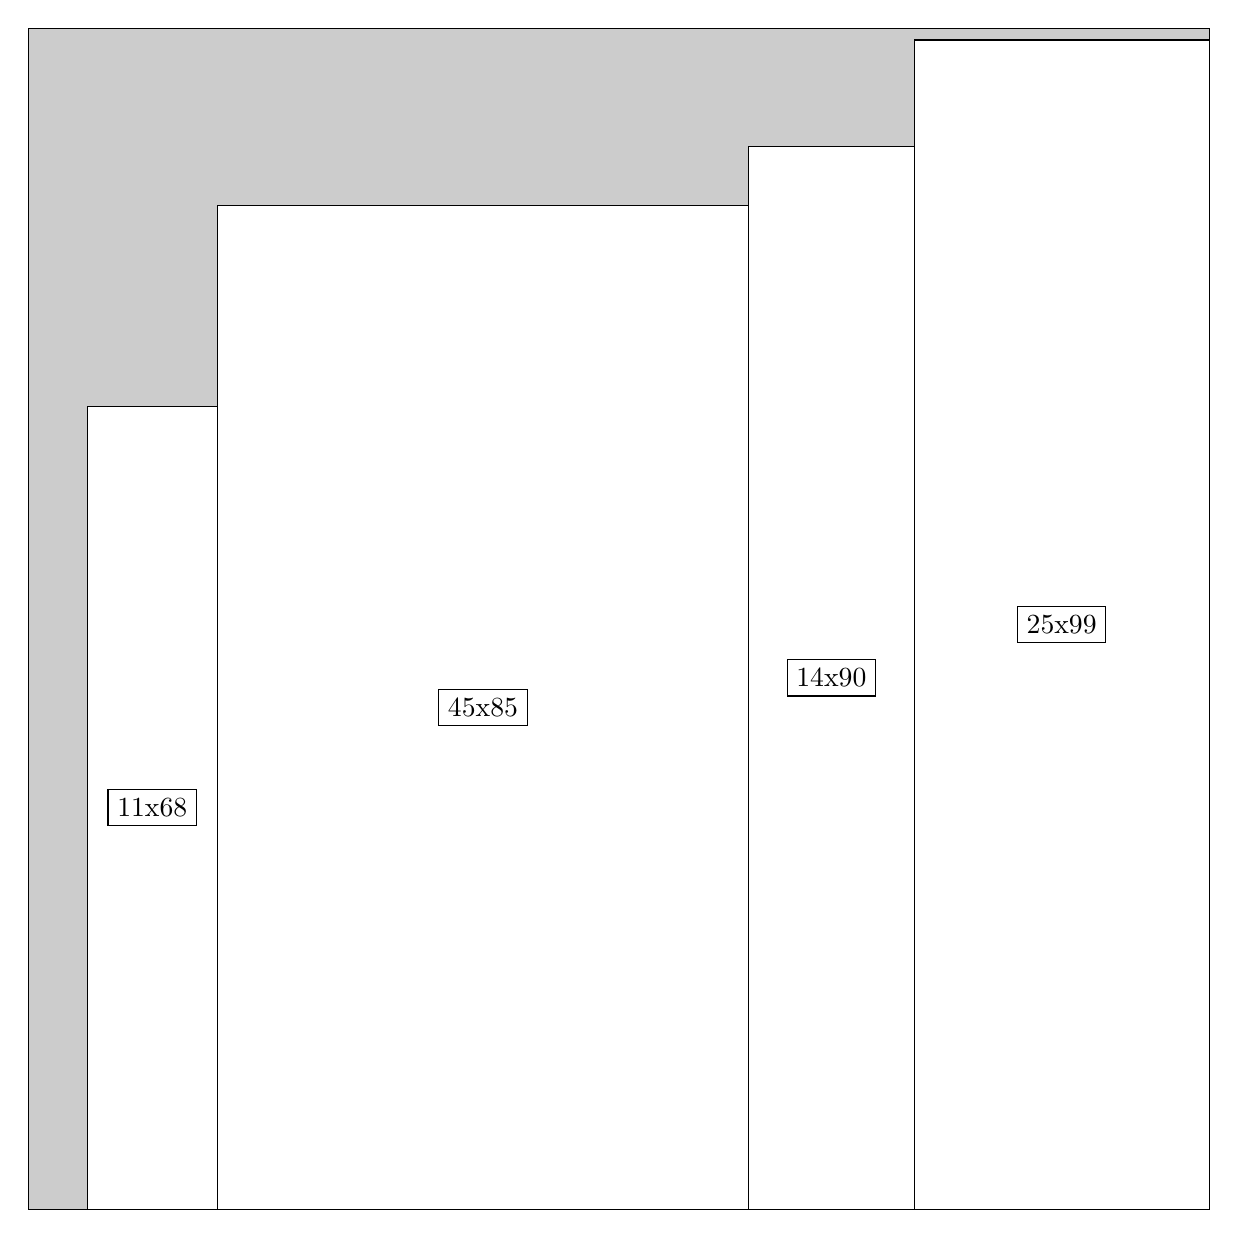
\begin{tikzpicture}[shorten >=1pt,scale=1.0,every node/.style={scale=1.0},->]
\tikzstyle{vertex}=[circle,fill=black!25,minimum size=14pt,inner sep=0pt]
\filldraw[fill=gray!40!white, draw=black] (0,0) rectangle (15.0,15.0);
\foreach \name/\x/\y/\w/\h in {25x99/11.25/0.0/3.75/14.85,14x90/9.15/0.0/2.1/13.5,45x85/2.4/0.0/6.75/12.75,11x68/0.75/0.0/1.65/10.2}
\filldraw[fill=white!40!white, draw=black] (\x,\y) rectangle node[draw] (\name) {\name} ++(\w,\h);
\end{tikzpicture}


w =25 , h =99 , x =75 , y =0 , v =2475
\par
w =14 , h =90 , x =61 , y =0 , v =1260
\par
w =45 , h =85 , x =16 , y =0 , v =3825
\par
w =11 , h =68 , x =5 , y =0 , v =748
\par
\newpage


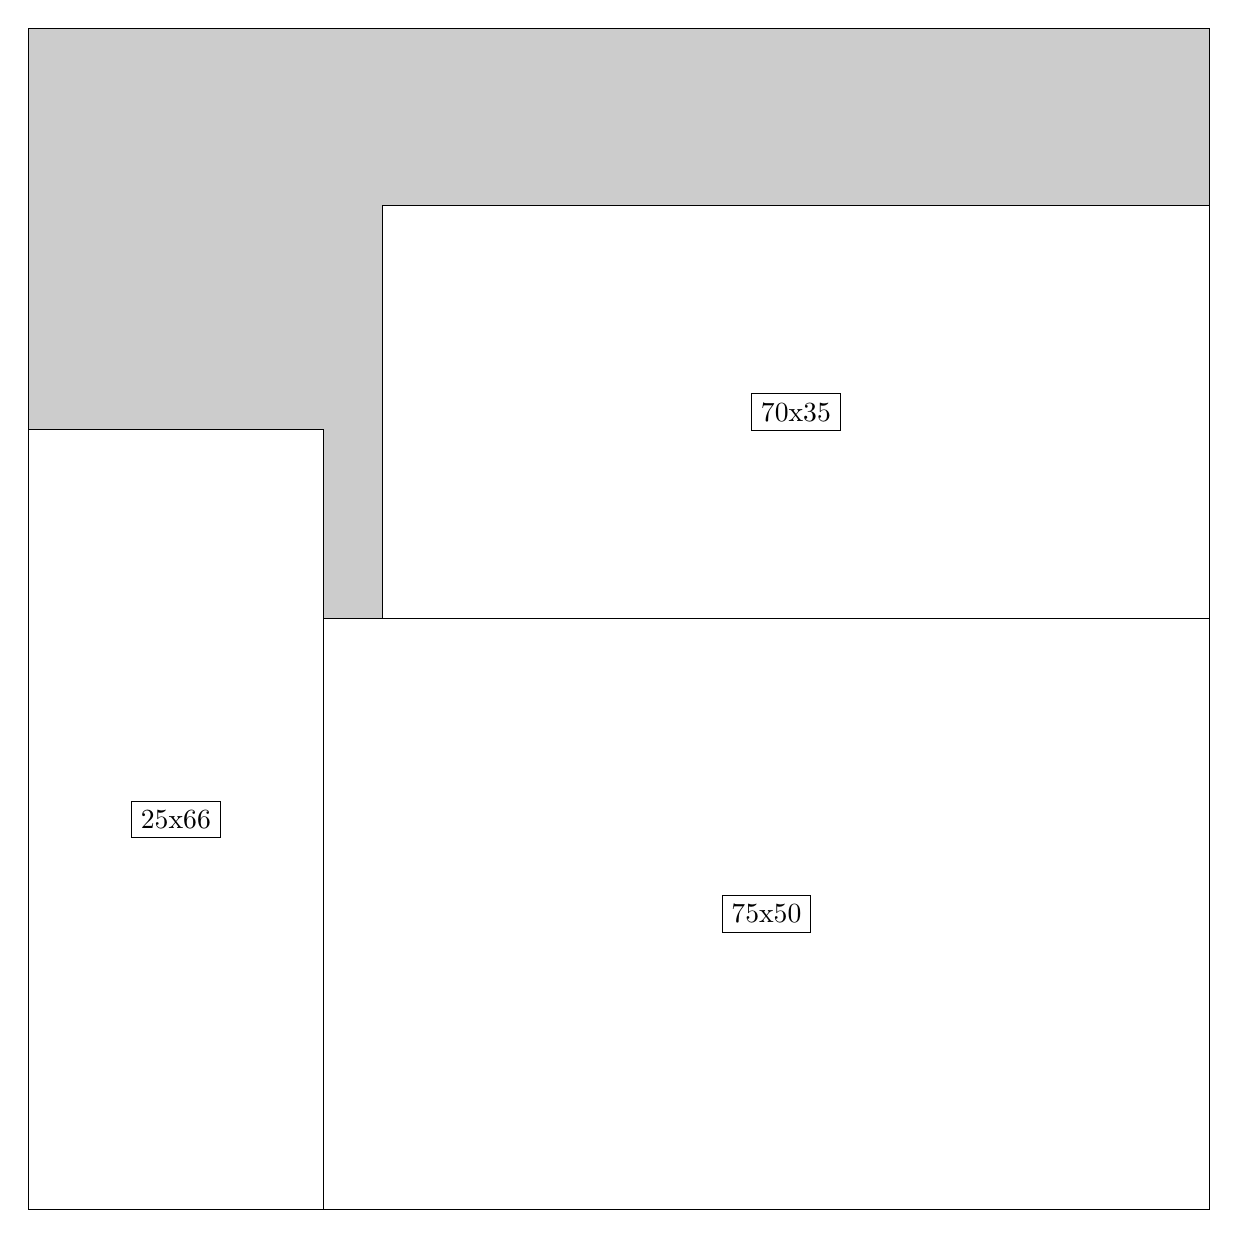
\begin{tikzpicture}[shorten >=1pt,scale=1.0,every node/.style={scale=1.0},->]
\tikzstyle{vertex}=[circle,fill=black!25,minimum size=14pt,inner sep=0pt]
\filldraw[fill=gray!40!white, draw=black] (0,0) rectangle (15.0,15.0);
\foreach \name/\x/\y/\w/\h in {75x50/3.75/0.0/11.25/7.5,70x35/4.5/7.5/10.5/5.25,25x66/0.0/0.0/3.75/9.9}
\filldraw[fill=white!40!white, draw=black] (\x,\y) rectangle node[draw] (\name) {\name} ++(\w,\h);
\end{tikzpicture}


w =75 , h =50 , x =25 , y =0 , v =3750
\par
w =70 , h =35 , x =30 , y =50 , v =2450
\par
w =25 , h =66 , x =0 , y =0 , v =1650
\par
\newpage


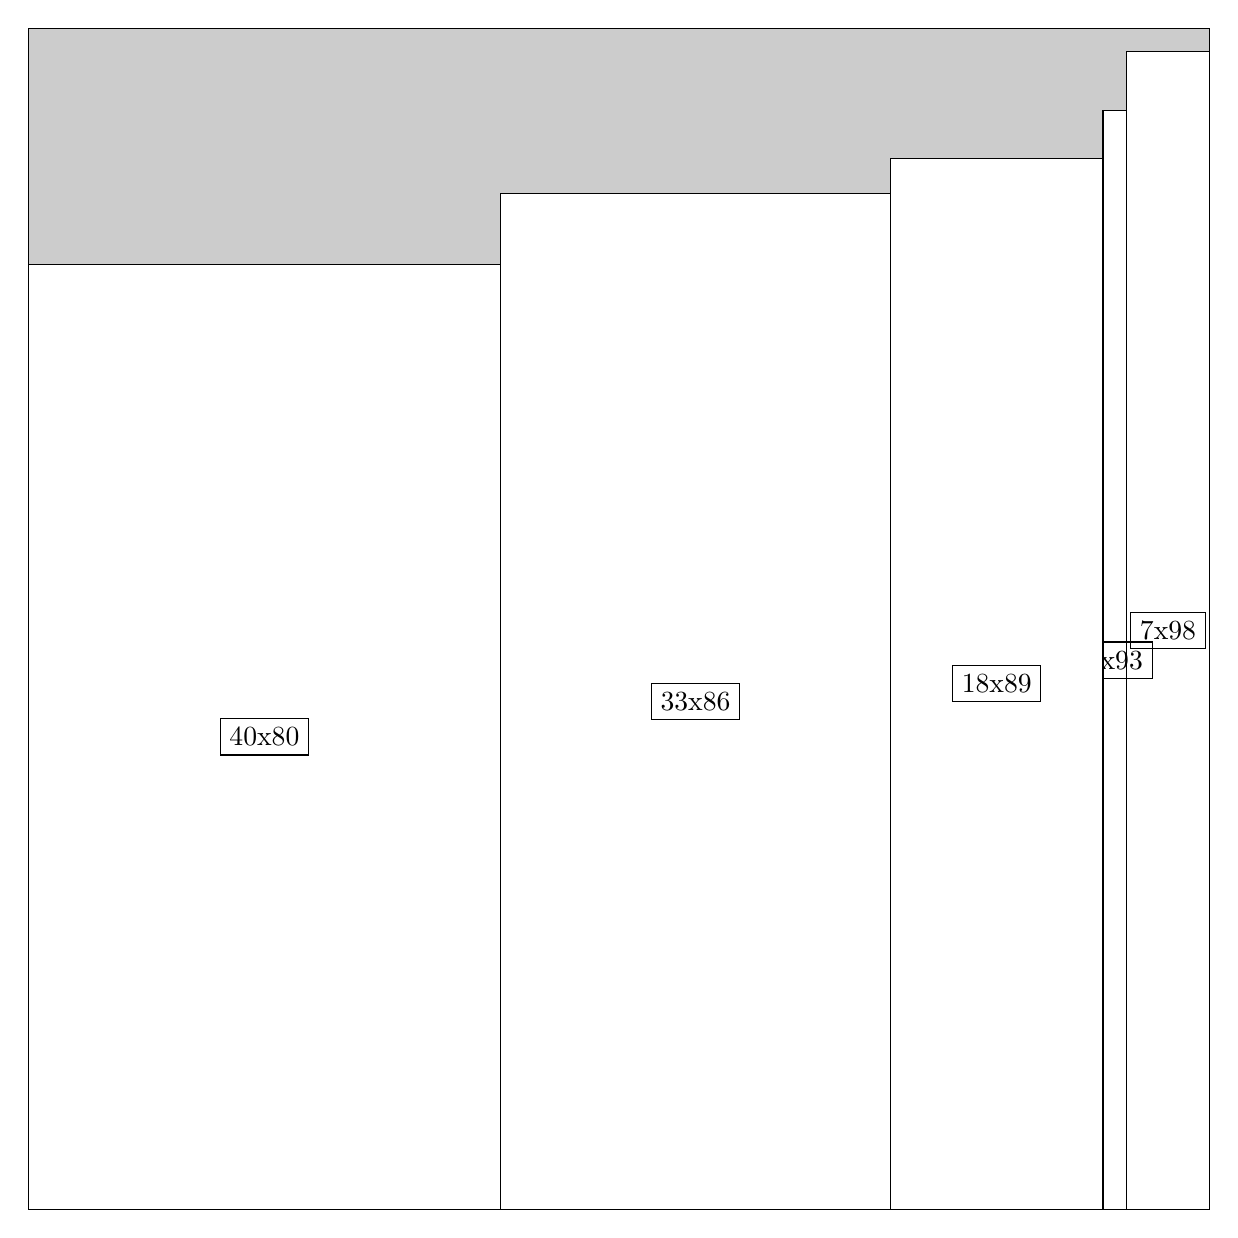
\begin{tikzpicture}[shorten >=1pt,scale=1.0,every node/.style={scale=1.0},->]
\tikzstyle{vertex}=[circle,fill=black!25,minimum size=14pt,inner sep=0pt]
\filldraw[fill=gray!40!white, draw=black] (0,0) rectangle (15.0,15.0);
\foreach \name/\x/\y/\w/\h in {7x98/13.95/0.0/1.05/14.7,2x93/13.65/0.0/0.3/13.95,18x89/10.95/0.0/2.6999999999999997/13.35,33x86/6.0/0.0/4.95/12.9,40x80/0.0/0.0/6.0/12.0}
\filldraw[fill=white!40!white, draw=black] (\x,\y) rectangle node[draw] (\name) {\name} ++(\w,\h);
\end{tikzpicture}


w =7 , h =98 , x =93 , y =0 , v =686
\par
w =2 , h =93 , x =91 , y =0 , v =186
\par
w =18 , h =89 , x =73 , y =0 , v =1602
\par
w =33 , h =86 , x =40 , y =0 , v =2838
\par
w =40 , h =80 , x =0 , y =0 , v =3200
\par
\newpage


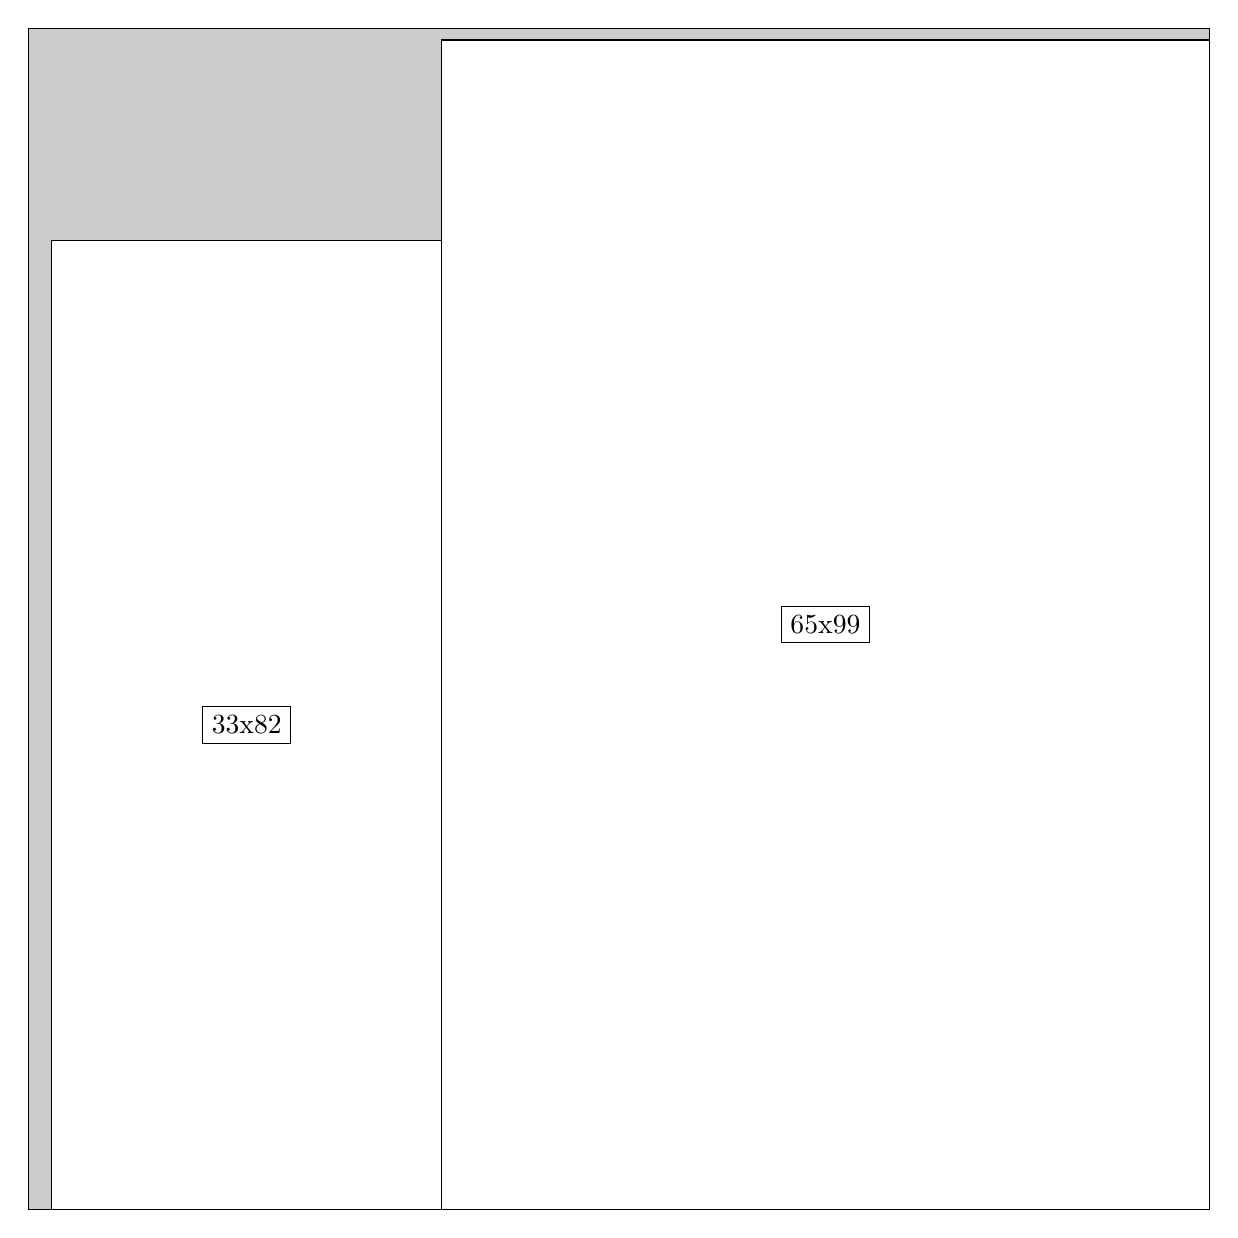
\begin{tikzpicture}[shorten >=1pt,scale=1.0,every node/.style={scale=1.0},->]
\tikzstyle{vertex}=[circle,fill=black!25,minimum size=14pt,inner sep=0pt]
\filldraw[fill=gray!40!white, draw=black] (0,0) rectangle (15.0,15.0);
\foreach \name/\x/\y/\w/\h in {65x99/5.25/0.0/9.75/14.85,33x82/0.3/0.0/4.95/12.299999999999999}
\filldraw[fill=white!40!white, draw=black] (\x,\y) rectangle node[draw] (\name) {\name} ++(\w,\h);
\end{tikzpicture}


w =65 , h =99 , x =35 , y =0 , v =6435
\par
w =33 , h =82 , x =2 , y =0 , v =2706
\par
\newpage


\end{document}